\section[Morphismen]{Morphismen und Isomorphismen von Spielen}\label{sec:Morphismen}

\todo[inline]{Motivation: Warum betrachtet man überhaupt Morphismen von Spielen. Wie induzieren diese Isomorphismen?}

Mögliche Motivationen:
\begin{itemize}
	\item Jedes Potential definiert selbst wieder ein Spiel mit einer gemeinsamen Kostenfunktion für alle Spieler. Und in einem gewissen Sinne ist dieses Spiel \glqq äquivalent\grqq zum ursprünglichen Spiel (z.B. gleiche Gleichgewichtspunkte). Das Hin- und Herwechseln zwischen diesen beiden Versionen eines Spiels kann man durch Morphismen beschreiben und die Äquivalenz der beiden wird dann dadurch sichtbar, dass diese Morphismen \emph{Isomorphismen} sind.
	\item Die Äquivalenz zwischen exakten Potentialspielen und Auslastungsspielen wird durch Morphismen beschrieben.
	\item Kategorientheoretische Sicht: Um eine Kategorie (hier: die der Spiele) zu verstehen, muss man ihre Morphismen kennen. Kennt man diese, so ergeben sich aus diesen auf natürliche Weise weitere Begriffe wie Isomorphismen von Spielen, Summen oder Produkte von Spielen.
\end{itemize}

\todo[inline]{Diese Punkte (insbesondere den letzten) näher ausführen?}

\subsection{Definitionen}

Zu zwei gegebenen Spielen $\Gamma = (I, X, (K_i)_{i\in I}, (c_i)_{i\in I})$ und $\Gamma' = (I', X', (K'_i)_{i\in I'}, (c'_i)_{i\in I})$ kann man wie folgt eine Abbildung zwischen diesen beiden definieren:
\begin{itemize}
	\item Eine bijektive Abbildung $\sigma: I \to I'$ zwischen den Spielermengen und
	\item für jeden Spieler $i \in I$ eine Abbildung $\phi_i: X_i \to X'_{\sigma(i)}$ seiner Strategien.
\end{itemize}
\cite{Polyequilibrium} bezeichnet derartige Abbildungen \emph{Strategieersetzungsvorschriften}.\todo{Mehr dazu schreiben - erst später bei rationalen SEVs erwähnen?}

\begin{beob}
	Mit dieser Definition ist es also nur möglich Abbildungen zwischen Spielen mit Spielermengen gleicher Kardinalität zu definieren. Im Folgenden werden wir ausschließlich solche Abbildungen betrachten (vergleiche aber \Cref{bem:LapMorDef} dazu wie auch in anderen Fällen Abbildungen zwischen Spielen definiert werden können). Zur Vereinfachung der Notation werden wir daher ab sofort immer davon ausgehen, dass die Spielermengen beider an einer Abbildung beteiligten Spiele bereits gleich und geeignet permutiert sind.
\end{beob}

Abbildungen der obigen Form nehmen noch keinerlei Rücksicht auf die Kostenfunktionen der jeweiligen Spiele. Da diese aber in der Regel die interessierenden Eigenschaften eines Spiels (wie beispielsweise Gleichgewichte) festlegen, werden derartige Abbildungen im Allgemeinen noch wenig Aussagen über die beteiligten Spiele ermöglichen. So besagt der durch diese Art Abbildungen induzierte Isomorphiebegriff bspw. nur, dass zwei Spiele Spieler- und Strategiemengen gleicher Kardinalität besitzen.

Echte Morphismen zwischen Spielen sollten folglich noch mehr der Struktur eines Spiels erhalten, insbesondere in irgendeiner Form \glqq verträglich\grqq{} mit den Kostenfunktionen sein. Je nach dem, welche Eigenschaften die Morphismen (und insbesondere die dadurch induzierten Isomorphismen) erhalten sollen, erhält man so unterschiedlich starke Einschränkungen daran, welche Abbildungen zwischen Spielen als \emph{Morphismen zwischen Spielen} bezeichnet werden dürfen. Einige Möglichkeiten dafür werden wir nun kennenlernen.

Eine relative starke Forderung ist die, dass Morphismen \emph{kostenerhaltend} sein müssen, wie sie in \cite{ReprOfFiniteGamesAsNCG} gestellt wird:

\begin{defn}
	Ein Morphismus $\phi$ von $\Gamma = (I, X, (K_i)_{i\in I}, (c_i)_{i\in I})$ nach $\Gamma' = (I, X', (K_i)_{i\in I}, (c'_i)_{i\in I})$ heißt \emph{kostenerhaltend}, wenn für alle Strategieprofile $x \in X$ und jeden Spieler $i \in I$ gilt:
		\[c_i(x) = c'_i(\phi(x)) \]
	Ist ein solcher Morphismus gleichzeitig ein Isomorphismus, so nennen wir $\Gamma$ und $\Gamma'$ \emph{äquivalent}.
\end{defn}

\begin{bem}
	Zwei Spiele sind also genau dann äquivalent, wenn sie sich ausschließlich durch Umbenennung der Strategien ineinander überführen lassen. In \cite{MonShap} (S. 133) wird dies als Isomorphie von Spielen bezeichnet.
\end{bem}

Eine auf das Untersuchen von Nash- und Polygleichgewichten zugeschnittene Form von Morphismen wird in \cite{Polyequilibrium} wie folgt definiert\todo{dort allerdings nur für Endomorphismen definiert}:

\begin{defn}
	Ein Morphismus $\phi$ von $\Gamma = (I, X, (K_i)_{i\in I}, (c_i)_{i\in I})$ nach $\Gamma' = (I, X', (K'_i)_{i\in I}, (c'_i)_{i\in I})$ heißt \emph{rational}, wenn für alle Strategieprofile $x \in X$, jeden Spieler $i \in I$ und jede Strategie $x'_i \in X'_i$ gilt:
	\[c'_i(\phi(x)) \leq c'_i(\phi_{-i}(x_{-i}), x'_i) \]
\end{defn}

\todo[inline]{Ist diese Definition sinnvoll/zielführend?}

\begin{defn}\label{def:SpielIsomLap}
	Zwei Spiele $\Gamma = (I, X, (K_i)_{i\in I}, (c_i)_{i\in I})$ und $\Gamma' = (I, X', (K'_i)_{i\in I}, (c'_i)_{i\in I})$ heißen \emph{isomorph}, falls es bijektive Abbildungen $\phi_i: X_i \to X'_i$ sowie bijektive und monotone Abbildungen $\psi_i: K_i \to K'_i$ gibt, sodass alle Diagramme der folgenden Form kommutieren:
	
	\begin{center}
		\begin{tikzcd}
			X \rar{\phi} \dar{c_i} & X' \dar{c'_i} \\
			K_i \rar{\psi_i}		& K'_i
		\end{tikzcd}
	\end{center}
\end{defn}

\begin{bem}\label{bem:LapMorDef}
	Diese Definition ergibt sich aus der abstrakteren Definition für \todo{...} in \cite{LapGameCat}. 
	
	\todo[inline]{Auch auf Verallgemeinerung mit Garben hinweisen (erlaubt Abbildungen zwischen Spielen mit Spielermengen unterschiedlicher Kardinalität!)}
\end{bem}

\begin{defn}
	Zwei im Sinne von \Cref{def:SpielIsomLap} isomorphe Spiele heißen \emph{sozial isomorph}, wenn zusätzlich die Funktion
		\[\sum \psi_i: \prod_{i \in I}K_i \to \prod_{i \in I} K'_i \]
	monoton ist. \todo{Das macht natürlich nur Sinn, wenn auf den beiden Produkträumen auch totale (?) Ordnungen existieren}
\end{defn}

\begin{bsp}
	lineare Funktionen
\end{bsp}	

Eine ganze Familie von Morphismen erhält man zudem aus den in \Cref{sec:Potentiale} beschriebenen Potentialen: \citeauthor{ReprOfFiniteGamesAsNCG} definiert in \cite{ReprOfFiniteGamesAsNCG} einen Isomorphismusbegriff der dazu führt, dass jedes exakte Potentialspiel isomorph zu dem Spiel ist, bei dem die Potentialfunktion als für alle Spieler einheitliche Kostenfunktion verwendet wird. Analog hierzu lassen sich auch für die anderen Potentialbegriffe passende Begriffe eines Morphismus (und damit eines Isomorphismus) definieren:

\begin{defn}\label{def:PotentialMorphismen}
	Ein Morphismus $\phi$ von $\Gamma = (I, X, (K_i)_{i\in I}, (c_i)_{i\in I})$ nach $\Gamma' = (I, X', (K'_i)_{i\in I}, (c'_i)_{i\in I})$ heißt
	\begin{itemize}
		\item \emph{exakt}, wenn für alle Strategieprofile $x \in X$, Spieler $i \in I$ und Strategien $\hat{x}_i$ gilt:
			\[c_i(x) - c_i(x_{-i}, \hat{x}_i) = c'_i(\phi(x)) - c'_i(\phi(x_{-i}, \hat{x}_i))\]
		\item \emph{gewichtend}, wenn es einen Vektor $(w_i)_{i \in I}$ gibt, sodass für alle Strategieprofile $x \in X$, Spieler $i \in I$ und Strategien $\hat{x}_i$ gilt:
			\[c_i(x) - c_i(x_{-i}, \hat{x}_i) = w_i\cdot\left(c'_i(\phi(x)) - c'_i(\phi(x_{-i}, \hat{x}_i))\right)\]
		\item \emph{skalierend}, wenn es streng monotone Funktionen $f_i$ gibt, sodass für alle Strategieprofile $x \in X$, Spieler $i \in I$ und Strategien $\hat{x}_i$ gilt:
			\[c_i(x) - c_i(x_{-i}, \hat{x}_i) = f_i(c'_i(\phi(x)) - c'_i(\phi(x_{-i}, \hat{x}_i)))\]
		\item \emph{ordinal}, wenn für alle Strategieprofile $x \in X$, Spieler $i \in I$ und Strategien $\hat{x}_i$ gilt:
			\[c_i(x) < c_i(x_{-i}, \hat{x}_i) \implies c'_i(\phi(x)) < c'_i(\phi(x_{-i}, \hat{x}_i))\]
		\item \emph{beste Antwort-erhaltend}, wenn für alle Spieler $i \in I$ und Strategieprofile $x_{-i} \in X_{-i}$ gilt:
			\[\phi(\arg \min_{x_i \in X_i}c_i(x)) \subseteq \arg \min_{x'_i \in X'_i} c'_i(\phi_{-i}(x_{-i}), x'_i)\]
	\end{itemize}	
\end{defn}

\begin{bem}
	Umgekehrt könnte man nun auch ausgehend von diesen Morphismen-Begriffen definieren, wann ein Spiel ein Potentialspiel ist: Ein Spiel ist nämlich genau dann ein exaktes/gewichtetes/ordinales/beste-Antwort-Potentialspiel, wenn es exakt/gewichtet/ordinal isomorph zu einem Spiel mit einer gemeinsamen Kostenfunktion für alle Spieler ist. Ein Spiel hat genau dann ein verallgemeinertes ordinales Potential, wenn es einen ordinalen Morphismus in ein solches Spiel gibt.
\end{bem}

\todo[inline]{Zu beste Antwort: vgl. \cite{FictPlayProp}, \cite{BestRespEq}}

\todo[inline]{Induzieren diese Morphismen jetzt wirklich die behaupteten Isomorphismen?}

\begin{beob}
	Es gelten folgende Beziehungen zwischen den verschiedenen Morphismenbegriffen:
	\begin{center}
		kostenerhaltend $\implies$ exakt $\implies$ gewichtend $\implies$ skalierend $\implies$ ordinal
		
		rational $\implies$ beste Antwort-erhaltend
		
		
	\end{center}
	\todo[inline]{weitere Zusammenhänge? Evtl. dann als Diagramm?}
\end{beob}


\begin{bem}
	Ein alternativer Ansatz zur Definition von Morphismen von Spielen verwendet \citeauthor{Foundations} in \cite{Foundations}. Darin werden einzelne Strategien nicht zwangsläufig wieder auf einzelne Strategien abgebildet, sondern können gleich auf ganze Teilmengen des Bildstrategieraums abgebildet werden. Von diesem Morphismentyp werden dann verschiedene \glqq approximativ kostenerhaltende\grqq{} Varianten betrachtet und die sich dadurch ergebende Kategorie studiert.
\end{bem}


\subsection{Erste Sätze}

\begin{prop}\label{prop:ordMorphVerbPf}
	Sei $\phi: \Gamma \to \Gamma'$ ein ordinaler Morphismus und $x^0, x^1, \dots$ ein Verbesserungspfad in $\Gamma$. Dann ist $\phi(x^0), \phi(x^1), \dots$ ein Verbesserungspfad in $\Gamma'$. Ist der Pfad endlich und in $\Gamma'$ abgeschlossen, so auch in $\Gamma$.
\end{prop}

\begin{proof}
	Da Morphismen spielerweise definiert sind, erhalten sie die Eigenschaft der unilateralen Abweichung. Die Ordinalität des Morphismus stellt ferner sicher, dass jeder Verbesserungsschritt ein Verbesserungsschritt bleibt.
	
	Nehmen wir nun an $\phi(x^0), \dots, \phi(x^n)$ wäre ein abgeschlossener Verbesserungspfad in $\Gamma'$, aber $x^0, \dots, x^n$ nicht abgeschlossen in $\Gamma$. Dann gäbe es folglich ein Strategieprofil $x^{n+1} \in X$, welches diesen Pfad in $\Gamma$ verlängert. Aber wie wir gerade gezeigt haben wäre dann auch $\phi(x^0), \dots, \phi(x^n), \phi(x^{n+1})$ ein Verbesserungspfad in $\Gamma'$, insbesondere also eine Verlängerung des ursprünglichen Pfades - im Widerspruch zu dessen vorausgesetzter Abgeschlossenheit.
\end{proof}

\begin{kor}
	Ordinale Morphismen reflektieren Nash-Gleichgewichte. Das heißt, ist $x \in X$ ein Strategieprofil in $\Gamma$ und $\phi$ ein ordinaler Morphismus in ein Spiel $\Gamma'$, sodass $\phi(x)$ ein Nash-Gleichgewicht in diesem ist, dann war bereits $x$ ein Nash-Gleichgewicht von $\Gamma$.
\end{kor}

\begin{proof}
	Es ist $x$ ein trivialer Verbesserungspfad in $\Gamma$, dessen Bild $\phi(x)$ in $\Gamma'$ abgeschlossen ist. Daher ist mit \Cref{prop:ordMorphVerbPf}  $x$ in $\Gamma$ abgeschlossen und folglich (vgl. \Cref{beob:VerbPfadeundNGe}) $x$ ein Nash-Gleichgewicht in $\Gamma$.
\end{proof}

\begin{kor}
	Seien $\Gamma$ und $\Gamma'$ zwei ordinal-isomorphe Spiele. Dann ist $x \in X$ genau dann ein Nashgleichgewicht von $\Gamma$, wenn $\phi(x) \in X'$ ein Nashgleichgewicht von $\Gamma'$ ist.
\end{kor}

Ordinal-isomorphe Spiele haben also die gleichen Nash-Gleichgewichte. Selbiges gilt auch für Verbesserungpfade, das heißt insbesondere, dass die FIP eines Spiels unter ordinaler Isomorphie erhalten bleibt.

\begin{kor}
	Seien $\Gamma$ und $\Gamma'$ zwei ordinal-isomorphe Spiele. Dann hat $\Gamma$ genau dann die FIP, wenn $\Gamma'$ diese besitzt.
\end{kor}


\begin{lemma}
	Seien $\Gamma$ und $\Gamma'$ zwei sozial isomorphe Spiele. Dann ist $x \in X$ genau dann ein soziales Optimum von $\Gamma$, wenn $\phi(x) \in X'$ ein soziales Optimum von $\Gamma'$ ist.
\end{lemma}

\begin{proof}
	.
	
	\todo[inline]{Folgt direkt mit Definitionen}
\end{proof}

\begin{satz}
	Besitzt ein Spiel $\Gamma$ ein ordinales Potential, so ist es ordinal-isomorph zu einem Auslastungsspiel.
\end{satz}

\begin{proof}
	Analog zum Beweis der Äquivalenz von Spielen mit exaktem Potential und Auslastungsspielen in \cite{MonShap}, Beweis orientiert sich an \cite{MultiPotGames}.
\end{proof}

\begin{beob}
	Besitzt ein Spiel ein verallgemeinertes ordinales Potential, so gibt es einen ordinalen Morphismus in/von \todo{Was von beidem?} ein Auslastungsspiel.
\end{beob}

\begin{proof}
	.
	\todo[inline]{Proofmining in oberem Beweis}
\end{proof}

\begin{beob}
	Nach \cite{MonShap} Lemma 2.5 hat jedes Spiel mit FIP ein verallgemeinertes Potential, also \todo[inline]{in/von...}
\end{beob}


\subsection{Überblick}

\begin{figure}[h]\centering
	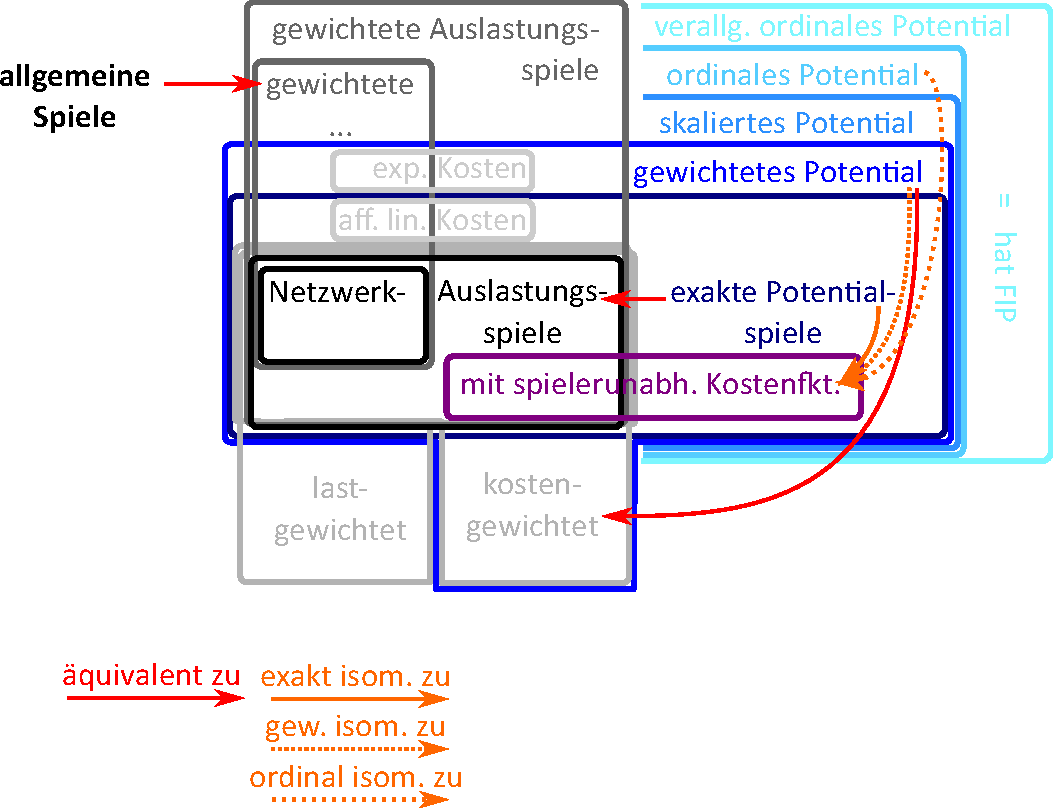
\includegraphics[width=.7\textwidth]{../Bilder/VennDiagramm.pdf}
	\caption{Zusammenhänge zwischen den verschiedenen Spieleklassen}
\end{figure}